\chapter[AUTOSAR]{\thechapter. AUTOSAR}
\section{Overview}
The design architecture used in AUTOSAR represents the layered pattern\footnote{Automobil-Elektornik - January 2007 - S.28} using a component-based approach. One of the key benefits of this kind of architecture, which is applied extensively in software development, are the well-defined interfaces and strong dependency management.\newline
\begin{center}
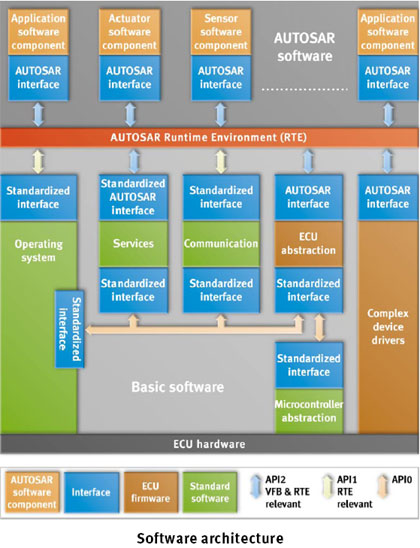
\includegraphics[scale=0.60]{Images/autosar_arch.jpg}\\
\end{center}
Because of the broad scope and variety of software layers presented in AUTOSAR architecture as show above, the scope of this case study will be modeling of the memory stack. The main reason for this decision is that the memory stack is to be found in every automotive unit.\footnote{Leitner Fl. Evaluation of the Matlab Simulink Design Verier versus the model checker, S. 24}\newpage
\section{Memory stack }
The memory stack is divided into three main components: Memory service, Memory hardware abstraction, Memory drivers.
\begin{center}
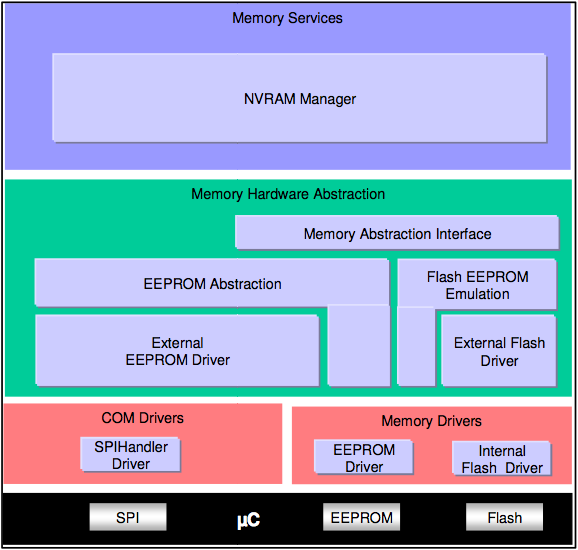
\includegraphics[scale=0.60]{Images/Figure2_1.png}\\
\end{center}
The memory stack is to be initial by the Operation System (OS) and the request operation are managed by the AUTOSAR Runtime Environment (RTE).\newpage
\subsection{Memory service}
The NVRAM component contains of two main components. They shall provides specific services according to their individual requirements. In particular there is a data management and a maintenance component. The maintenance component is responsible for all loading, writting and saving processes. The data management component is responsible for maintaining  of the non-volite data. Further more these component communicates with the RTE, OS, MemIf, EcuM,DEM,DET and CRC Library. 
\subsection{Memory hardware abstraction}
The contains three components
\begin{itemize}
\item Memory abstraction interface (MemIf) acts like a router, that manages the request made by the NvM
\item Flash eeprom emulator (Fee) takes control over the flash driver
\item EEPROM abstraction (Ea) takes control over the eeprom driver
\end{itemize}
\subsection{Memory drivers}
The contains three components
\begin{itemize}
\item Flash driver (Fls)
\item Eeprom driver (Eee)
\item Vendor specific driver (Vsd)
\end{itemize}